\documentclass[a4paper,french]{report}
\usepackage{geometry,babel,graphicx,lineno,pdfpages}
\usepackage[T1]{fontenc}
\usepackage[utf8]{inputenc}
\usepackage[color links=true,link color=black]{hyperref}
\graphicspath{{./figs/}}
\makeatletter
%% meta function
\def\make@object#1{\expandafter\gdef\csname#1\endcsname{\object{#1}}}
\newcommand{\object}[1]{\texttt{#1}}
\make@object{forecast}
\make@object{bank}
\make@object{liquid}
\make@object{saving}
\newcommand{\catForecast}[1]{\textsf{#1}}

\makeatother

\begin{document}

\author{Sylvain}
\date{Compilé le \today}
\title{Compta \theversion}

\pagenumbering{alph}
\maketitle

\pagenumbering{arabic}
\tableofcontents
\newpage

{\it%
Une comptabilité saine consiste à classer chaque opération
dont on veut garder une trace. Ce programme permet de
sauvegarder, classer et traiter des opérations de comptabilité
traditionnelle, c'est-à-dire des flux d'argent entre les liquidités,
un ou plusieurs compte en banques, un ou plusieurs compte épargnes,
le tout classer et traiter suivant un schéma prévisionnel.

Plus simplement, l'ensemble des dépenses que l'on opère se
classent dans différentes catégories, par exemple un loyer pourra être considéré
comme une dépense dans une catégorie \og Dépenses fixes\fg ou 
\og Administratif\fg, et les dépenses courantes pour la nourriture dans
une catégorie \og Vie courante\fg ou \og Inévitable\fg,\dots

Chacune de ces catégories va donc représenter une certaine somme
dépensée tous les mois, ce qui permet d'allouer à cette catégorie
une somme au début du mois. Une comptabilité comparera l'état
des dépenses effectuées à un certain moment avec les provisions
prévues, et donc permet de garder un \oe il sur l'état des
finances.

Ce programme se propose de tracer l'ensemble des flux d'argent,
en traitant l'ensemble des opérations par rapport à des prévisions,
les suivant entre le liquides, un ou des comptes en banque et comptes
d'épargne. Ainsi on a une estimation précise de l'argent restant dans le/les
compte(s) et en poche.
}


\chapter{Fonctionnement}
\label{chap:func}
\section{Les objets}
Les instances prises en compte sont le prévisionnel
(\forecast), le compte en banque (\bank) et le 
liquide disponible (\liquid). Une opération est un flux d'argent, 
entrant ou sortant du compte ou du liquide. Les combinaisons possibles 
sont entre le compte et le liquide, ou à l'intérieur du compte entre le 
compte courant et un ou plusieurs compte-épargne (\saving).

Une prévision se fait sur un pas de temps prédéfinis, les sommes
étant prévues pour une période fixe. Cette période est par convention
dans ce programme le mois.

\subsection{Prévisionnel}

Prévoir les dépenses peut se faire en les classant et assignant
un plafond à ne pas dépasser. La prédiction étant un art difficile,
et surtout lorsqu'il s'agit du futur\footnote{\og Prediction is very
difficult, especially about the futur.\fg\ \textsc{Niels Bohr}
(1885--19620)}, ce plafond peut se nuancer d'une certaine marge
pour le rendre flottant.
Ainsi chaque catégorie se caractérise par un nom, un plafond, mais
aussi une marge de man\oe uvre.

Il est possible (et même fortement probable) qu'il existe des
opérations récurrentes tous les mois, typiquement des factures, 
un loyer, un prêt, etc\dots\ Ainsi il faut pouvoir ajouter
à certaines catégories des opérations qui, par hypothèse,
se passeront à un moment ou un autre dans le mois.
Donc il est possible d'ajouter des opérations dans chaque
catégorie.

Le prévisionnel se décompose en catégories. Le but étant de classer 
l'ensemble des opérations par catégorie, de définir un plafond par 
catégorie et de comparer les dépenses et recettes réelles aux 
provisions allouées à la catégorie. Une catégorie peut comprendre 
des opérations attendues, comme par exemple un prêt ou un loyer à 
payer, ou n'importe quel prélèvement automatique.

\begin{figure}[htp]
\centering
\includegraphics[width=\linewidth]{forecast}
\caption{\label{forecast}Forecast}
\end{figure}

\subsection{Compte bancaire}
\subsection{Compte épargne}
\subsection{Liquide}


\label{sec:object}

\chapter{Fichier d'entrée}
\section{Exemple complet}
\footnotesize
\begin{verbatim}
Longjumeau comptabilité
EUR
#Date           Category        Amount  Margin   sub cat, automatic, date start, date end
forecast        Prêt            627.71  0.00   Prêt taux 1, PA, 15/01/2012
forecast        Prêt            151.61  10.00   Prêt taux 2, PA, 15/01/2012
forecast        Assurance       300.00  150.00              , PNA
forecast        Téléphonie      2.00    0.00   Free Mobile, PA, 10/01/2012, 10/01/2015, 2
forecast        Téléphonie      4.77    0.00   OVH,         PA, 01/01/2012
forecast        Cadeaux         5.00    0.00   MSF,                PA, 01/01/2012
forecast        Cadeaux         6.00    0.00   AIDES,              PA, 01/01/2012
forecast        Cadeaux         7.00    0.00   CARE,               PA, 01/01/2012
forecast        Cadeaux         6.00    0.00   ADECE,              PA, 01/01/2012
forecast        Cadeaux         10.00   0.00   Secours Catholique, PA, 01/01/2012
forecast        Administratif   218.06  0.00   Appel de fonds Syndic,          PA, 01/01/2012
forecast        Administratif   30.00   0.00   virement Epargne Illyana,       PA, 01/01/2012
forecast        Administratif   2.40    0.00   Cotisation CNV Equipage Facile, PA, 01/01/2012
forecast        Administratif   5.40    0.00   Cotisation CNV Equipage 2,      PA, 01/01/2012
forecast        Administratif   3.62    0.00   Cotisation CNV Co-Equipage 2,   PA, 01/01/2012
forecast        Administratif   30.00   0.00   Assurance vie Sylvain,          PA, 01/01/2012
forecast        Administratif   500.00  150.00   , PNA
# Account       dependance         amount  start_date   name            , currency (if different)
bank            main               918.57  01/01/2012   BPVF
savings         BPVF                 0.00  01/01/2012   livret A enfants
savings         BPVF                 0.00  01/01/2012   Epargne Illyana
bank            other                0.00  01/01/2012   BoA             , USD
cash            main                 3.09  01/01/2012   liquide France
#Date           Category        Debit   Credit  Identifier  Liquide Operation
20/04/2012      Cadeaux         50.00   0.00    Bn      Chèque 239 mariage Olivia et JM
05/05/2012      Administratif   5.00    0.00    B       Youpi glop zork glups
16/05/2012      Administratif   82.00   0.00    B       Graaaak namok
16/05/2012      Administratif   24.26   0.00    B       Blurp
01/06/2012      Administratif   2.40    0.00    B       Cotisation CNV Equipage Facile
05/06/2012      Cadeaux         5.00    0.00    B       MSF
05/06/2012      Cadeaux         7.00    0.00    B       CARE
05/06/2012      Administratif   3.62    0.00    B       Cotisation CNV Co-Equipage 2
05/06/2012      Administratif   30.00   0.00    B       Assurance vie Sylvain
05/06/2012      Administratif   30.00   0.00    B       Plan Epargne Enfant Illyana
08/06/2012      Administratif   0.00    250.00  V       livret A enfants
08/06/2012      Administratif   25.00   0.00    V       liquide France
11/06/2012      Cadeaux         10.00   0.00    B       Secours Catholique
12/06/2012      Administratif   5.40    0.00    B       Cotisation CNV Equipage 2
12/06/2012      Téléphonie      6.95    0.00    B       OVH
13/06/2012      Administratif   402.66  0.00    V       BoA, 500 USD
13/06/2012      Administratif   0.00    500.00  V       livret A enfants
14/06/2012      Prêt            627.71  0.00    B       Prêt taux 1
14/06/2012      Prêt            151.61  0.00    B       Prêt taux 2
15/06/2012      Administratif   218.06  0.00    B       Appel de fonds Syndic
15/06/2012      Administratif   17.90   0.00    B       Appel de fonds Syndic pour clôture
20/06/2012      Cadeaux         6.00    0.00    B       ADECE
20/06/2012      Cadeaux         6.00    0.00    B       AIDES
20/06/2012      Téléphonie      2.00    0.00    B       Free Mobile
20/06/2012      Administratif   0.00    300.00  V       livret A enfants
\end{verbatim}
\normalsize


\section{Entête}
\linenumbers
\footnotesize
\begin{verbatim}
Longjumeau comptabilité
EUR
\end{verbatim}
\nolinenumbers

Les premières lignes sont simplement le titre pour la sortie \LaTeX\
et la monnaie à utiliser.


\section{Prévisionnel}
\linenumbers
\footnotesize
\begin{verbatim}
#Date           Category        Amount  Margin   sub cat, automatic, date start, date end
forecast        Prêt            627.71  0.00   Prêt taux 1, PA, 15/01/2012
forecast        Prêt            151.61  10.00   Prêt taux 2, PA, 15/01/2012
forecast        Assurance       300.00  150.00              , PNA
forecast        Téléphonie      2.00    0.00   Free Mobile, PA, 10/01/2012, 10/01/2015, 2
forecast        Téléphonie      4.77    0.00   OVH,         PA, 01/01/2012
forecast        Cadeaux         5.00    0.00   MSF,                PA, 01/01/2012
forecast        Cadeaux         6.00    0.00   AIDES,              PA, 01/01/2012
forecast        Cadeaux         7.00    0.00   CARE,               PA, 01/01/2012
forecast        Cadeaux         6.00    0.00   ADECE,              PA, 01/01/2012
forecast        Cadeaux         10.00   0.00   Secours Catholique, PA, 01/01/2012
forecast        Administratif   218.06  0.00   Appel de fonds Syndic,          PA, 01/01/2012
forecast        Administratif   30.00   0.00   virement Epargne Illyana,       PA, 01/01/2012
forecast        Administratif   2.40    0.00   Cotisation CNV Equipage Facile, PA, 01/01/2012
forecast        Administratif   5.40    0.00   Cotisation CNV Equipage 2,      PA, 01/01/2012
forecast        Administratif   3.62    0.00   Cotisation CNV Co-Equipage 2,   PA, 01/01/2012
forecast        Administratif   30.00   0.00   Assurance vie Sylvain,          PA, 01/01/2012
forecast        Administratif   500.00  150.00   , PNA
\end{verbatim}
\nolinenumbers
\normalsize


\section{Comptes}
\linenumbers
\footnotesize
\begin{verbatim}
# Account       dependance         amount  start_date   name            , currency (if different)
bank            main               918.57  01/01/2012   BPVF
savings         BPVF                 0.00  01/01/2012   livret A enfants
savings         BPVF                 0.00  01/01/2012   Epargne Illyana
bank            other                0.00  01/01/2012   BoA             , USD
cash            main                 3.09  01/01/2012   liquide France
\end{verbatim}
\nolinenumbers
\normalsize


\section{Données}
\linenumbers
\footnotesize
\begin{verbatim}
#Date           Category        Debit   Credit  Identifier  Liquide Operation
20/04/2012      Cadeaux         50.00   0.00    Bn      Chèque 239 mariage Olivia et JM
05/05/2012      Administratif   5.00    0.00    B       Youpi glop zork glups
16/05/2012      Administratif   82.00   0.00    B       Graaaak namok
16/05/2012      Administratif   24.26   0.00    B       Blurp
01/06/2012      Administratif   2.40    0.00    B       Cotisation CNV Equipage Facile
05/06/2012      Cadeaux         5.00    0.00    B       MSF
05/06/2012      Cadeaux         7.00    0.00    B       CARE
05/06/2012      Administratif   3.62    0.00    B       Cotisation CNV Co-Equipage 2
05/06/2012      Administratif   30.00   0.00    B       Assurance vie Sylvain
05/06/2012      Administratif   30.00   0.00    B       Plan Epargne Enfant Illyana
08/06/2012      Administratif   0.00    250.00  V       livret A enfants
08/06/2012      Administratif   25.00   0.00    V       liquide France
11/06/2012      Cadeaux         10.00   0.00    B       Secours Catholique
12/06/2012      Administratif   5.40    0.00    B       Cotisation CNV Equipage 2
12/06/2012      Téléphonie      6.95    0.00    B       OVH
13/06/2012      Administratif   402.66  0.00    V       BoA, 500 USD
13/06/2012      Administratif   0.00    500.00  V       livret A enfants
14/06/2012      Prêt            627.71  0.00    B       Prêt taux 1
14/06/2012      Prêt            151.61  0.00    B       Prêt taux 2
15/06/2012      Administratif   218.06  0.00    B       Appel de fonds Syndic
15/06/2012      Administratif   17.90   0.00    B       Appel de fonds Syndic pour clôture
20/06/2012      Cadeaux         6.00    0.00    B       ADECE
20/06/2012      Cadeaux         6.00    0.00    B       AIDES
20/06/2012      Téléphonie      2.00    0.00    B       Free Mobile
20/06/2012      Administratif   0.00    300.00  V       livret A enfants
\end{verbatim}
\nolinenumbers
\normalsize


\appendix
\chapter{Sortie pdf de l'exemple}
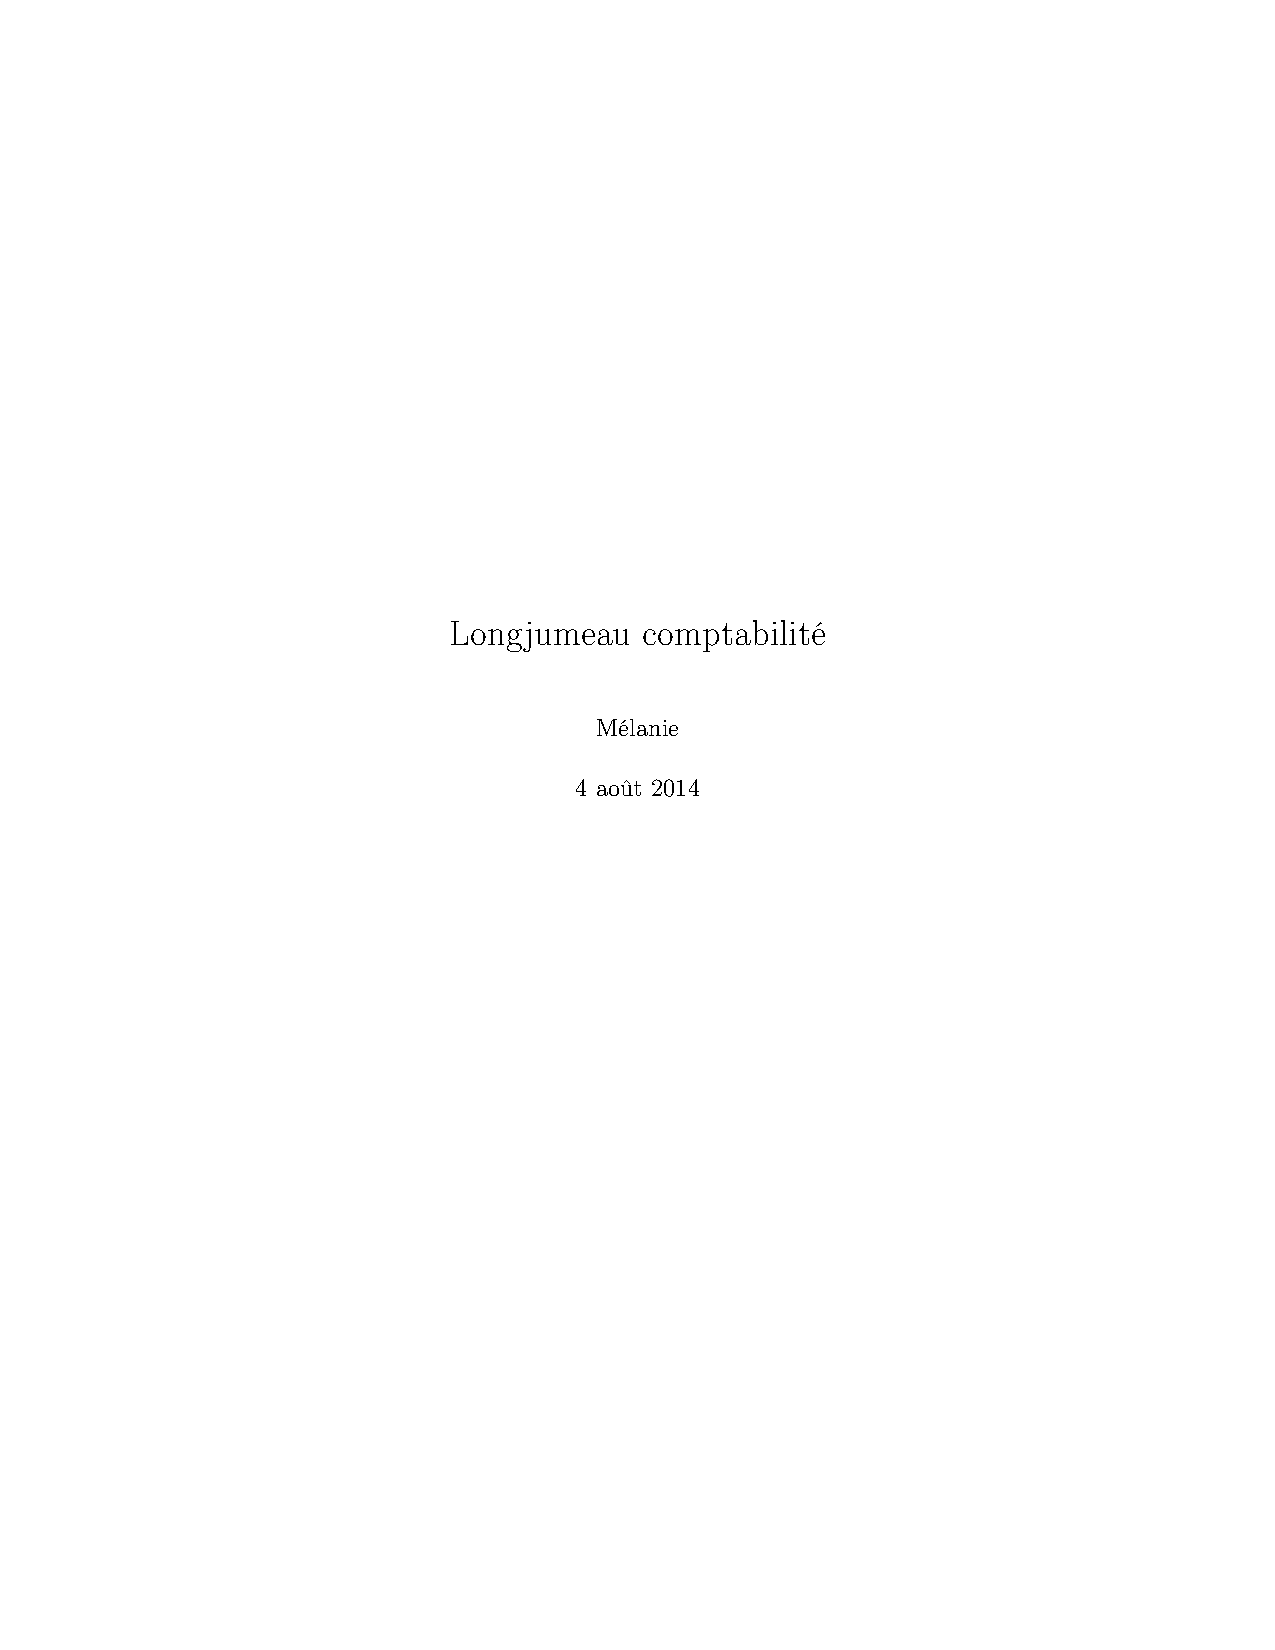
\includepdf[pages=-]{./figs/Longjumeau_data}

\end{document}
